\documentclass[../../Instruction_PupilCapture]{subfiles}
% Hier müssen keine Packages geladen werden, es werden automatisch die von masterdoc geladen,
% sowie die Konfigurationen.
\graphicspath{{img/}{img/}}
\begin{document}

\chapter{Usage of Pupil Capture}
The following is a short instruction how use Pupil Capture in conjunction with the framework.

\begin{enumerate}
	\item Select \textit{Unity Stream} as Capture Selection in the world window and activate the Unity Capture (Figure \ref{fig:screenshot001}).
	
	\begin{figure}[htp]
		\centering
		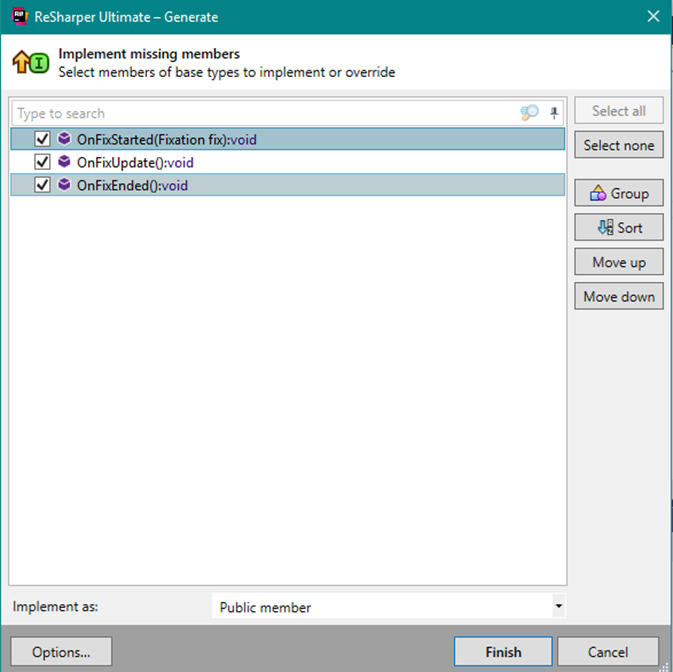
\includegraphics[width=0.5\linewidth]{img/screenshot001}
		\caption{Section \textit{Capture Selection} for use of \textit{Unity Stream}}
		\label{fig:screenshot001}
	\end{figure}
	\begin{figure}[htp]
		\centering
		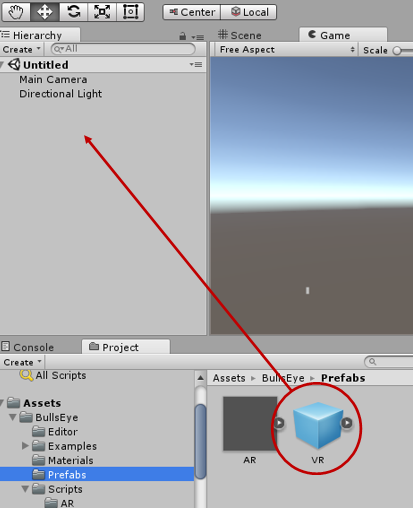
\includegraphics[width=0.5\linewidth]{screenshot003}
		\caption{Selected \textit{Unity Stream} and click on \textit{Activate Unity Capture}}
		\label{fig:screenshot003} 
	\end{figure}
	\item Open an eye window by activating \textit{Detect Eye 0} or \textit{Detect Eye 1}. Use one for monocular eye tracking or two for binocular (Figure \ref{fig:screenshot002}). Check the \textit{detection \& mapping mode} is on \textit{2d}.
	\begin{figure}[htp]
		\centering
		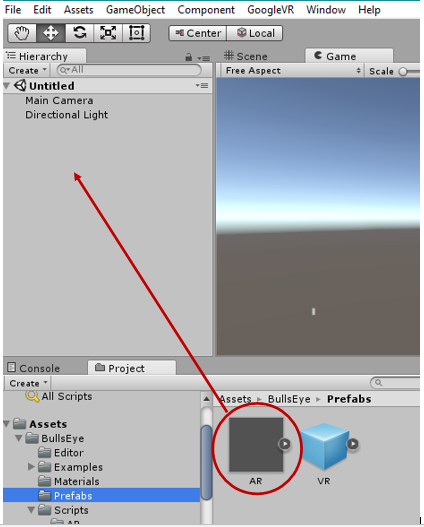
\includegraphics[width=0.5\linewidth]{screenshot002}
		\caption{General settings with the one eye activated for monocular eye tracking}
		\label{fig:screenshot002}
	\end{figure}
	\item Select the USB camera for eye tracking by selecting \textit{Local USB} as Capture Selection in the eye window. Afterwards select the camera in the \textit{Activate source} list (Figure \ref{fig:screenshot004}).
	\begin{figure}[h!]
		\centering
		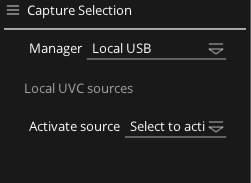
\includegraphics[width=0.5\linewidth]{screenshot004}
		\caption{Activating \textit{Local USB} in on the eye window}
		\label{fig:screenshot004}
	\end{figure}\clearpage
	\item Now set the mode to \textit{ROI} in the general settings of the eye window (Figure \ref{fig:screenshot005}). After this the test person look to the left, to the right, up and down. Decrease the size of the  shown rectangle while the pupil has to be always inside of the rectangle. You can change the size of the rectangle by grabbing the circles in the corners. Figure \ref{roi} shows how the rectangle should be fitted around the eye.
	\begin{figure}[h!]
		\centering
		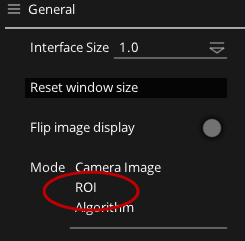
\includegraphics[width=0.5\linewidth]{img/screenshot005}
		\caption{Select Mode \textit{ROI}}
		\label{fig:screenshot005}
	\end{figure}
	\begin{figure}[h!]
		\centering
		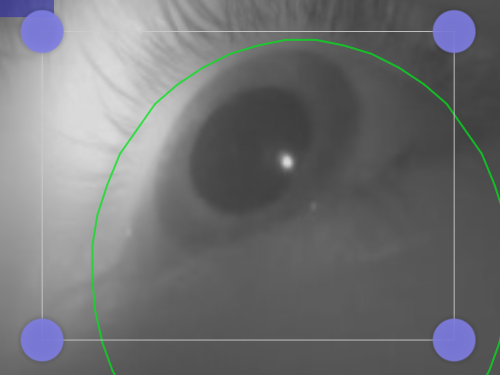
\includegraphics[width=0.5\linewidth]{ROI}
		\caption{The rectangle fitted around the eye}
		\label{roi}
	\end{figure}\clearpage
	\item Test which settings for \textit{Pupil intensity range}, \textit{Pupil min}, and \textit{Pupil max} result in the most accurate eye tracking by using the slider (Figure \ref{PupilSettings})  		
	\begin{figure}[h!]
		\centering
		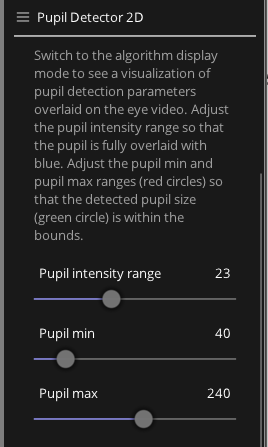
\includegraphics[scale=0.8]{PupilSettings.png}
		\caption{The settings for the pupil detection}
		\label{PupilSettings}
	\end{figure}
	\item For calibrating the eye tracking you have to switch over to the world window. Choose the right calibration (\textit{Manual Marker Calibration}) as shown in figure \ref{fig:screenshot006}.
	\begin{figure}[h!]
		\centering
		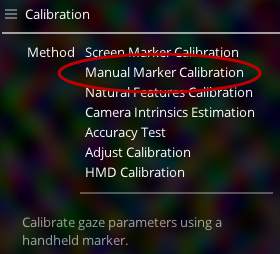
\includegraphics[width=0.5\linewidth]{img/screenshot006}
		\caption{Selection calibration method}
		\label{fig:screenshot006}
	\end{figure}
	Then press the left button (\textit{X}) on the remote control and let the test person look around to place the appeared marker in the center of the screen.
	\item Click the \textit{C} on the left hand side of the world window or use the \textit{c} key to start the calibration. Now a small circle will appear in the upper left hand corner (Figure \ref{Calibration}) and fill itself when the marker is detected and the subject looking at it.
	\begin{figure}[h!]
		\centering
		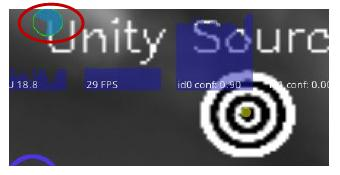
\includegraphics[width=0.8\linewidth]{img/Calibration}
		\caption{The circle indicating during the calibration}
		\label{Calibration}
	\end{figure}
	\item Every time the circle is full, press the left button (\textit{X} on the remote control) again, to move the marker to the next position. After nine positions, click \textit{C} again to complete the calibration. You can press the right button (triangle) to make the marker disappear.
	\item Check the accuracy and repeat the calibration if necessary.
\end{enumerate}

\end{document}